% Môn: Toán
% Lớp: 10
% Chương: Chương I. Mệnh đề và tập hợp
% Bài: Bài 2. Tập hợp và các phép toán trên tập hợp · Ứng dụng sơ đồ Venn và bài toán thực tế về tập hợp
% Số câu: 56
% App đọc file này trực tiếp — sửa rồi Commit trên GitHub, bấm Đồng bộ GitHub .tex

% Bài 2. Tập hợp và các phép toán trên tập hợp

% ===== Câu 1 =====
% ID: T10C1B2-01-DS
% Mức: TH
\dangbt{Ứng dụng sơ đồ Venn và bài toán thực tế về tập hợp}
\begin{ex}
% ID: T10C1B2-01-DS
% Mức: THXét các phát biểu sau về số lượng học sinh tham gia các câu lạc bộ trong lớp $10C6$: Lớp $10C6$ có $18$ học sinh tham gia câu lạc bộ bóng đá và $15$ học sinh tham gia câu lạc bộ bóng rổ. Biết rằng có $10$ học sinh tham gia cả hai câu lạc bộ trên.
\choiceTF
{ Có $8$ học sinh tham gia ít nhất một trong hai câu lạc bộ trên.}
{\True Có $23$ học sinh tham gia ít nhất một trong hai câu lạc bộ trên.}
{Biết lớp $10C6$ có $45$ học sinh. Có $25$ học sinh không tham gia câu lạc bộ bóng đá.}
{Biết lớp $10C6$ có $45$ học sinh. Có $24$ học sinh không tham gia cả hai câu lạc bộ.}
\loigiai{
Gọi $A$ là tập hợp học sinh tham gia câu lạc bộ bóng đá, $B$ là tập hợp học sinh tham gia câu lạc bộ bóng rổ.
Theo đề bài, ta có: $|A| = 18$, $|B| = 15$, $|A \cap B| = 10$.
a) Số học sinh tham gia ít nhất một trong hai câu lạc bộ là số phần tử của tập hợp $A \cup B$. Ta có công thức:
$|A \cup B| = |A| + |B| - |A \cap B||A \cup B| = 18 + 15 - 10 = 33 - 10 = 23$.
Phát biểu "Có $8$ học sinh tham gia ít nhất một trong hai câu lạc bộ trên" là Sai.
b) Dựa trên kết quả tính toán ở câu a), số học sinh tham gia ít nhất một trong hai câu lạc bộ là $23$.
Phát biểu "Có $23$ học sinh tham gia ít nhất một trong hai câu lạc bộ trên" là Đúng.
c) Gọi $L$ là tập hợp học sinh lớp $10C6$. Theo đề bài, $|L| = 45$.
Số học sinh không tham gia câu lạc bộ bóng đá là số học sinh thuộc lớp $10C6$ nhưng không thuộc tập $A$. Số này được tính bằng $|L| - |A|$.
Số học sinh không tham gia câu lạc bộ bóng đá là $45 - 18 = 27$.
Phát biểu "Biết lớp $10C6$ có $45$ học sinh. Có $25$ học sinh không tham gia câu lạc bộ bóng đá" là Sai.
d) Gọi $L$ là tập hợp học sinh lớp $10C6$. Theo đề bài, $|L| = 45$.
Số học sinh không tham gia cả hai câu lạc bộ là số học sinh thuộc lớp $10C6$ nhưng không thuộc tập $A \cup B$. Số này được tính bằng $|L| - |A \cup B|$.
Từ câu a), ta có $|A \cup B| = 23$.
Số học sinh không tham gia cả hai câu lạc bộ là $45 - 23 = 22$.
Phát biểu "Biết lớp $10C6$ có $45$ học sinh. Có $24$ học sinh không tham gia cả hai câu lạc bộ" là Sai.
}
\end{ex}

% ===== Câu 10 =====
% ID: T10C1B2-03-TL
% Mức: VD
\begin{bt}
% ID: T10C1B2-03-TL
% Mức: VD
Lớp 10 $A$ có $45$ học sinh trong đó có $25$ em học giỏi môn Toán, $23$ em học giỏi môn Lý, $20$ em học giỏi môn Hóa, $11$ em học giỏi cả môn Toán và môn Lý, $8$ em học giỏi cả môn Lý và môn Hóa, $9$ em học giỏi cả môn Toán và môn Hóa. Hỏi lớp $10A$ có bao nhiêu bạn học giỏi cả ba môn Toán, Lý, Hóa? (biết rằng mỗi học sinh trong lớp học giỏi ít nhất một trong ba môn Toán, Lý, Hóa).
\loigiai{
Gọi $T$, $L$, $H$ lần lượt là tập hợp học sinh giỏi môn Toán, Lý, Hóa.
Ta có công thức $|T \cup L \cup H| = |T| + |L| + |H| - |T \cap L| - |L \cap H| - |H \cap T| + |T \cap L \cap H|$.
Thay số: $45 = 25 + 23 + 20 - 11 - 8 - 9 + |T \cap L \cap H|$.
$\Leftrightarrow |T \cap L \cap H| = 45 - (25 + 23 + 20) + (11 + 8 + 9)$.
$\Leftrightarrow |T \cap L \cap H| = 45 - 68 + 28$.
$\Leftrightarrow |T \cap L \cap H| = 5$.
Vậy có 5 học sinh giỏi cả ba môn Toán, Lý, Hóa.
5
}
\end{bt}

% ===== Câu 11 =====
% ID: T10C1B2-03-TLN
% Mức: VD
\begin{ex}
% ID: T10C1B2-03-TLN
% Mức: VD
Một lớp học có $25$ học sinh chơi bóng đá, $23$ học sinh chơi bóng bàn, $14$ học sinh chơi cả bóng đá và bóng bàn, $6$ học sinh không chơi môn nào. Tìm số học sinh chỉ chơi một môn thể thao.
\shortans{20}
\loigiai{
Gọi $A$ là tập hợp các học sinh chơi bóng đá, $B$ là tập hợp các học sinh chơi bóng bàn, $C$ là tập hợp các học sinh không chơi môn thể thao nào.
Ta có
 $|A|$ là số học sinh chơi bóng đá;
$|B|$ là số học sinh chơi bóng bàn;
$|C|$ là số học sinh không chơi môn thể thao nào.
Khi đó số học sinh chỉ chơi một môn thể thao là:
 $|A|+|B|-2| A \cap B| = 25+23- 2 \cdot 14=20$.
}
\end{ex}

% ===== Câu 17 =====
% ID: T10C1B2-05-DS
% Mức: TH
\begin{ex}
% ID: T10C1B2-05-DS
% Mức: THXét lớp $10 B_1$ có $7$ học sinh giỏi Toán, $5$ học sinh giỏi Lý, $6$ học sinh giỏi Hóa. Trong đó, có $2$ học sinh chỉ giỏi Toán và Lý, $3$ học sinh chỉ giỏi Toán và Hóa, $1$ học sinh chỉ giỏi Lý và Hóa, và $1$ học sinh giỏi cả $3$ môn Toán, Lý, Hóa. Hãy nhận xét các phát biểu sau:
\choiceTF
{\True Số học sinh chỉ giỏi môn Toán là $1$.}
{\True Số học sinh chỉ giỏi môn Lý là $1$.}
{Số học sinh chỉ giỏi môn Hóa là $2$.}
{\True Số học sinh giỏi ít nhất một môn (Toán, Lý, Hóa) là $10$.}
\loigiai{
Gọi T, L, H lần lượt là tập hợp các học sinh giỏi Toán, Lý, Hóa.
Theo đề bài, ta có:
$|T| = 7|L| = 5|H| = 6|T \cap L \setminus H| = 2$ (chỉ giỏi Toán và Lý)
$|T \cap H \setminus L| = 3$ (chỉ giỏi Toán và Hóa)
$|L \cap H \setminus T| = 1$ (chỉ giỏi Lý và Hóa)
$|T \cap L \cap H| = 1$ (giỏi cả 3 môn)
a. Số học sinh chỉ giỏi môn Toán:
Số học sinh chỉ giỏi Toán là $ |T| - (|T \cap L \setminus H| + |T \cap H \setminus L| + |T \cap L \cap H|) $.
$ 7 - (2 + 3 + 1) = 7 - 6 = 1 $.
Vậy, phát biểu "Số học sinh chỉ giỏi môn Toán là $1$" là đúng.
b. Số học sinh chỉ giỏi môn Lý:
Số học sinh chỉ giỏi Lý là $ |L| - (|T \cap L \setminus H| + |L \cap H \setminus T| + |T \cap L \cap H|) $.
$ 5 - (2 + 1 + 1) = 5 - 4 = 1 $.
Vậy, phát biểu "Số học sinh chỉ giỏi môn Lý là $1$" là đúng.
c. Số học sinh chỉ giỏi môn Hóa:
Số học sinh chỉ giỏi Hóa là $ |H| - (|T \cap H \setminus L| + |L \cap H \setminus T| + |T \cap L \cap H|) $.
$ 6 - (3 + 1 + 1) = 6 - 5 = 1 $.
Vậy, phát biểu "Số học sinh chỉ giỏi môn Hóa là $2$" là sai (vì số học sinh chỉ giỏi Hóa là $1)$.
d. Số học sinh giỏi ít nhất một môn (Toán, Lý, Hóa):
Số học sinh giỏi ít nhất một môn là $ |T \cup L \cup H| $.
Áp dụng công thức hợp của ba tập hợp:
$ |T \cup L \cup H| = |T| + |L| + |H| - (|T \cap L| + |T \cap H| + |L \cap H|) + |T \cap L \cap H| $.
Ta có:
$ |T \cap L| = |T \cap L \setminus H| + |T \cap L \cap H| = 2 + 1 = 3 $.
$ |T \cap H| = |T \cap H \setminus L| + |T \cap L \cap H| = 3 + 1 = 4 $.
$ |L \cap H| = |L \cap H \setminus T| + |T \cap L \cap H| = 1 + 1 = 2 $.
Vậy, $ |T \cup L \cup H| = 7 + 5 + 6 - (3 + 4 + 2) + 1 $.
$ |T \cup L \cup H| = 18 - 9 + 1 = 10 $.
Vậy, phát biểu "Số học sinh giỏi ít nhất một môn (Toán, Lý, Hóa) là $10$" là đúng.
}
\end{ex}

% ===== Câu 19 =====
% ID: T10C1B2-05-TLN
% Mức: TH
\begin{ex}
% ID: T10C1B2-05-TLN
% Mức: THLớp $10A$ có $45$ học sinh. Trong đó, có $12$ học sinh giỏi Văn, $9$ học sinh giỏi Địa lí và $30$ học sinh không giỏi môn học nào trong hai môn Văn, Địa lí. Hỏi lớp $10A$ có bao nhiêu học sinh giỏi cả hai môn Văn và Địa lí?
\shortans{6}
\loigiai{
Số học sinh giỏi Văn hoặc giỏi Địa lí là $45 - 30=15$ (học sinh).
Số học sinh giỏi cả hai môn Văn và Địa lí là $12+9-15=6$ (học sinh).
}
\end{ex}

% ===== Câu 33 =====
% ID: T10C1B2-15-TN
% Mức: TH
\begin{ex}
% ID: T10C1B2-15-TN
% Mức: THCho các tập hợp $A, B, X$ được biểu diễn trong biểu đồ Venn như hình vẽ dưới đây. Khẳng định nào sau đây là $\textbf{sai}$?
\begin{center}
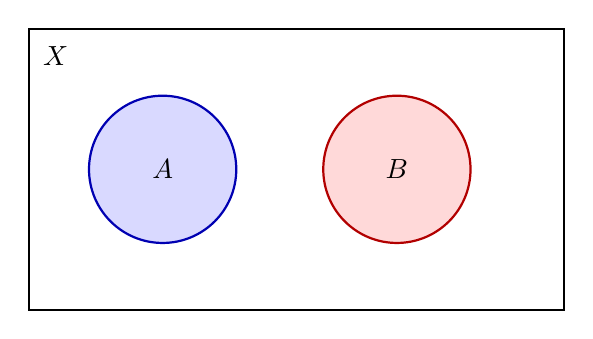
\begin{tikzpicture}[scale=0.85, every node/.style={font=\normalsize}]
    % Tập hợp X
    \draw[thick] (0,0) rectangle (8,4.2);
    \node at (0.4,3.8) {$X$};

    % Tập hợp A
    \draw[thick, blue!70!black, fill=blue!15]
        (2,2.1) circle (1.1);
    \node at (2,2.1) {$A$};

    % Tập hợp B
    \draw[thick, red!70!black, fill=red!15]
        (5.5,2.1) circle (1.1);
    \node at (5.5,2.1) {$B$};
\end{tikzpicture}
\end{center}
\choice
{$B \subset C_X A$}
{$A \cap B = \varnothing$}
{$A \subset C_X B$}
{\True $A \cup B = X$}
\loigiai{
Để xác định khẳng định sai, chúng ta sẽ phân tích từng phương án dựa trên biểu đồ Venn đã cho.
*   Phương án A:
    $C_X A$ là phần bù của $A$ trong $X$, tức là tập hợp các phần tử thuộc $X$ nhưng không thuộc $A$. Nhìn vào biểu đồ Venn, ta thấy toàn bộ tập hợp $B$ nằm hoàn toàn bên ngoài tập hợp $A$ và nằm trong $X$. Do đó, mọi phần tử của $B$ đều thuộc $C_X A$. Khẳng định $B \subset C_X A$ là đúng.
*   Phương án B:
    $A \cap B$ là giao của hai tập hợp $A$ và $B$, tức là tập hợp các phần tử chung của $A$ và $B$. Nhìn vào biểu đồ Venn, ta thấy tập hợp $A$ và tập hợp $B$ không có phần tử chung nào (hai hình tròn không giao nhau). Do đó, $A \cap B = \varnothing$. Khẳng định $A \cap B = \varnothing$ là đúng.
*   Phương án C:
    $C_X B$ là phần bù của $B$ trong $X$, tức là tập hợp các phần tử thuộc $X$ nhưng không thuộc $B$. Nhìn vào biểu đồ Venn, ta thấy toàn bộ tập hợp $A$ nằm hoàn toàn bên ngoài tập hợp $B$ và nằm trong $X$. Do đó, mọi phần tử của $A$ đều thuộc $C_X B$. Khẳng định $A \subset C_X B$ là đúng.
*   Phương án D:
    $A \cup B$ là hợp của hai tập hợp $A$ và $B$, tức là tập hợp các phần tử thuộc $A$ hoặc thuộc $B$ (hoặc cả hai). Nhìn vào biểu đồ Venn, ta thấy rằng có một phần của tập hợp $X$ nằm bên ngoài cả $A$ và $B$. Điều này có nghĩa là $A \cup B \neq X$. Khẳng định $A \cup B = X$ là sai.
Vậy, khẳng định sai là D.
}
\end{ex}
\begin{ex}
% Mức: TH
Một cửa hàng điện máy khảo sát $100$ khách hàng về việc mua tủ lạnh và máy giặt. Kết quả cho thấy có $60$ khách hàng mua tủ lạnh, $50$ khách hàng mua máy giặt, và $25$ khách hàng không mua cả hai sản phẩm. Hỏi có bao nhiêu khách hàng mua cả tủ lạnh và máy giặt?
\shortans{35}
\loigiai{Gọi $A$ là tập hợp khách hàng mua tủ lạnh, $B$ là tập hợp khách hàng mua máy giặt.
Ta có $|A| = 60$, $|B| = 50$.
Số khách hàng không mua cả hai sản phẩm là $25$, nên số khách hàng mua ít nhất một trong hai sản phẩm là $100 - 25 = 75$.
Theo công thức hợp của hai tập hợp: $|A \cup B| = |A| + |B| - |A \cap B|$.
Thay số vào, ta có $75 = 60 + 50 - |A \cap B|$.
$75 = 110 - |A \cap B|$.
$|A \cap B| = 110 - 75 = 35$.
Vậy có $35$ khách hàng mua cả tủ lạnh và máy giặt.}
\end{ex}

\begin{ex}
% Mức: TH
Đề: Một cuộc khảo sát về sở thích đọc sách của $100$ học sinh cho thấy: $45$ học sinh thích đọc truyện trinh thám, $38$ học sinh thích đọc truyện khoa học viễn tưởng, $32$ học sinh thích đọc truyện lịch sử. Có $15$ học sinh thích cả trinh thám và khoa học viễn tưởng, $12$ học sinh thích cả khoa học viễn tưởng và lịch sử, $10$ học sinh thích cả trinh thám và lịch sử. Biết rằng có $5$ học sinh thích đọc cả ba loại truyện trên. Hỏi có bao nhiêu học sinh không thích đọc bất kỳ loại truyện nào trong ba loại trên?
\loigiai{
Gọi $A$ là tập hợp học sinh thích đọc truyện trinh thám.
Gọi $B$ là tập hợp học sinh thích đọc truyện khoa học viễn tưởng.
Gọi $C$ là tập hợp học sinh thích đọc truyện lịch sử.
Theo đề bài, ta có:
$|A| = 45$
$|B| = 38$
$|C| = 32$
$|A \cap B| = 15$
$|B \cap C| = 12$
$|A \cap C| = 10$
$|A \cap B \cap C| = 5$
Số học sinh thích ít nhất một trong ba loại truyện là:
$|A \cup B \cup C| = |A| + |B| + |C| - (|A \cap B| + |B \cap C| + |A \cap C|) + |A \cap B \cap C|$
$|A \cup B \cup C| = 45 + 38 + 32 - (15 + 12 + 10) + 5$
$|A \cup B \cup C| = 115 - 37 + 5 = 83$
Tổng số học sinh được khảo sát là $100$.
Số học sinh không thích đọc bất kỳ loại truyện nào là:
$100 - |A \cup B \cup C| = 100 - 83 = 17$
Vậy có $17$ học sinh không thích đọc bất kỳ loại truyện nào trong ba loại trên.
}
\end{ex}

\begin{ex}
% Mức: TH
Đề: Trong một lớp học có $50$ học sinh, có $28$ học sinh tham gia câu lạc bộ bóng đá, $20$ học sinh tham gia câu lạc bộ bóng rổ, và $15$ học sinh tham gia câu lạc bộ cờ vua. Biết rằng có $10$ học sinh tham gia cả bóng đá và bóng rổ, $8$ học sinh tham gia cả bóng rổ và cờ vua, $6$ học sinh tham gia cả bóng đá và cờ vua. Có $3$ học sinh tham gia cả ba câu lạc bộ. Hỏi có bao nhiêu học sinh không tham gia câu lạc bộ nào?
\loigiai{
Gọi $B$ là tập hợp học sinh tham gia câu lạc bộ bóng đá.
Gọi $R$ là tập hợp học sinh tham gia câu lạc bộ bóng rổ.
Gọi $C$ là tập hợp học sinh tham gia câu lạc bộ cờ vua.
Theo đề bài, ta có:
$|B| = 28$
$|R| = 20$
$|C| = 15$
$|B \cap R| = 10$
$|R \cap C| = 8$
$|B \cap C| = 6$
$|B \cap R \cap C| = 3$
Số học sinh tham gia ít nhất một câu lạc bộ là:
$|B \cup R \cup C| = |B| + |R| + |C| - (|B \cap R| + |R \cap C| + |B \cap C|) + |B \cap R \cap C|$
$|B \cup R \cup C| = 28 + 20 + 15 - (10 + 8 + 6) + 3$
$|B \cup R \cup C| = 63 - 24 + 3 = 42$
Tổng số học sinh trong lớp là $50$.
Số học sinh không tham gia câu lạc bộ nào là:
$50 - |B \cup R \cup C| = 50 - 42 = 8$
Vậy có $8$ học sinh không tham gia câu lạc bộ nào.
}
\end{ex}

\begin{ex}
% Mức: TH
Đề: Một công ty tiến hành khảo sát $120$ nhân viên về việc sử dụng ba loại phần mềm $X, Y, Z$. Kết quả cho thấy: $60$ nhân viên sử dụng phần mềm $X$, $50$ nhân viên sử dụng phần mềm $Y$, $40$ nhân viên sử dụng phần mềm $Z$. Có $25$ nhân viên sử dụng cả $X$ và $Y$, $20$ nhân viên sử dụng cả $Y$ và $Z$, $15$ nhân viên sử dụng cả $X$ và $Z$. Biết rằng có $10$ nhân viên sử dụng cả ba phần mềm. Hỏi có bao nhiêu nhân viên chỉ sử dụng đúng một loại phần mềm?
\loigiai{
Gọi $X_s$ là tập hợp nhân viên sử dụng phần mềm $X$.
Gọi $Y_s$ là tập hợp nhân viên sử dụng phần mềm $Y$.
Gọi $Z_s$ là tập hợp nhân viên sử dụng phần mềm $Z$.
Theo đề bài, ta có:
$|X_s| = 60$
$|Y_s| = 50$
$|Z_s| = 40$
$|X_s \cap Y_s| = 25$
$|Y_s \cap Z_s| = 20$
$|X_s \cap Z_s| = 15$
$|X_s \cap Y_s \cap Z_s| = 10$
Số nhân viên chỉ sử dụng phần mềm $X$ là:
$|X_s| - (|X_s \cap Y_s| + |X_s \cap Z_s|) + |X_s \cap Y_s \cap Z_s|$
$= 60 - (25 + 15) + 10 = 60 - 40 + 10 = 30$
Số nhân viên chỉ sử dụng phần mềm $Y$ là:
$|Y_s| - (|X_s \cap Y_s| + |Y_s \cap Z_s|) + |X_s \cap Y_s \cap Z_s|$
$= 50 - (25 + 20) + 10 = 50 - 45 + 10 = 15$
Số nhân viên chỉ sử dụng phần mềm $Z$ là:
$|Z_s| - (|Y_s \cap Z_s| + |X_s \cap Z_s|) + |X_s \cap Y_s \cap Z_s|$
$= 40 - (20 + 15) + 10 = 40 - 35 + 10 = 15$
Tổng số nhân viên chỉ sử dụng đúng một loại phần mềm là:
$30 + 15 + 15 = 60$
Vậy có $60$ nhân viên chỉ sử dụng đúng một loại phần mềm.
}
\end{ex}

\begin{ex}
% Mức: TH
Trong một lớp học có 40 học sinh. Trong đó có 25 học sinh thích môn Toán, 20 học sinh thích môn Văn và 10 học sinh thích cả hai môn Toán và Văn. Hỏi có bao nhiêu học sinh không thích cả hai môn Toán và Văn?
\choice
{5 học sinh}
{\True 10 học sinh}
{15 học sinh}
{20 học sinh}
\loigiai{Gọi A là tập hợp các học sinh thích môn Toán, B là tập hợp các học sinh thích môn Văn.
Theo đề bài, ta có:
$|A| = 25$
$|B| = 20$
$|A \cap B| = 10$
Số học sinh thích ít nhất một trong hai môn là:
$|A \cup B| = |A| + |B| - |A \cap B| = 25 + 20 - 10 = 35$
Tổng số học sinh trong lớp là 40.
Số học sinh không thích cả hai môn Toán và Văn là:
$40 - |A \cup B| = 40 - 35 = 5$ học sinh.
Vậy có 5 học sinh không thích cả hai môn Toán và Văn.}
\nguon{https://notebooklm.google.com/notebook/1385ddba-8b2d-48c5-993a-c368fefa6b2e?utm_source=nlmm_share}
\end{ex}

\begin{ex}
% Mức: TH
Một lớp học có 30 học sinh. Trong đó có 18 học sinh giỏi Toán, 15 học sinh giỏi Văn và 8 học sinh giỏi cả Toán và Văn. Hỏi có bao nhiêu học sinh không giỏi môn nào trong hai môn Toán và Văn?
\choice
{3 học sinh}
{\True 5 học sinh}
{7 học sinh}
{9 học sinh}
\loigiai{Gọi T là tập hợp các học sinh giỏi Toán, V là tập hợp các học sinh giỏi Văn.
Theo đề bài, ta có:
$|T| = 18$
$|V| = 15$
$|T \cap V| = 8$
Số học sinh giỏi ít nhất một trong hai môn là:
$|T \cup V| = |T| + |V| - |T \cap V| = 18 + 15 - 8 = 25$
Tổng số học sinh trong lớp là 30.
Số học sinh không giỏi môn nào trong hai môn Toán và Văn là:
$30 - |T \cup V| = 30 - 25 = 5$ học sinh.
Vậy có 5 học sinh không giỏi môn nào trong hai môn Toán và Văn.}
\nguon{https://notebooklm.google.com/notebook/1385ddba-8b2d-48c5-993a-c368fefa6b2e?utm_source=nlmm_share}
\end{ex}

\begin{ex}
% Mức: TH
Trong một cuộc khảo sát về sở thích đọc sách của 100 người, có 60 người thích đọc truyện trinh thám, 45 người thích đọc truyện khoa học viễn tưởng và 20 người thích đọc cả hai loại truyện này. Hỏi có bao nhiêu người không thích đọc cả truyện trinh thám và truyện khoa học viễn tưởng?
\choice
{10 người}
{15 người}
{\True 20 người}
{25 người}
\loigiai{Gọi T là tập hợp những người thích đọc truyện trinh thám, K là tập hợp những người thích đọc truyện khoa học viễn tưởng.
Theo đề bài, ta có:
$|T| = 60$
$|K| = 45$
$|T \cap K| = 20$
Số người thích đọc ít nhất một trong hai loại truyện là:
$|T \cup K| = |T| + |K| - |T \cap K| = 60 + 45 - 20 = 85$
Tổng số người được khảo sát là 100.
Số người không thích đọc cả truyện trinh thám và truyện khoa học viễn tưởng là:
$100 - |T \cup K| = 100 - 85 = 15$ người.
Vậy có 15 người không thích đọc cả truyện trinh thám và truyện khoa học viễn tưởng.}
\nguon{https://notebooklm.google.com/notebook/1385ddba-8b2d-48c5-993a-c368fefa6b2e?utm_source=nlmm_share}
\end{ex}

\begin{ex}
% Mức: TH
Một lớp học có 45 học sinh. Trong đó có 28 học sinh thích bóng đá, 20 học sinh thích bóng chuyền và 12 học sinh thích cả bóng đá và bóng chuyền. Hỏi có bao nhiêu học sinh không thích môn thể thao nào trong hai môn trên?
\choice
{7 học sinh}
{\True 9 học sinh}
{11 học sinh}
{13 học sinh}
\loigiai{Gọi BĐ là tập hợp các học sinh thích bóng đá, BC là tập hợp các học sinh thích bóng chuyền.
Theo đề bài, ta có:
$|BĐ| = 28$
$|BC| = 20$
$|BĐ \cap BC| = 12$
Số học sinh thích ít nhất một trong hai môn thể thao là:
$|BĐ \cup BC| = |BĐ| + |BC| - |BĐ \cap BC| = 28 + 20 - 12 = 36$
Tổng số học sinh trong lớp là 45.
Số học sinh không thích môn thể thao nào trong hai môn trên là:
$45 - |BĐ \cup BC| = 45 - 36 = 9$ học sinh.
Vậy có 9 học sinh không thích môn thể thao nào trong hai môn trên.}
\nguon{https://notebooklm.google.com/notebook/1385ddba-8b2d-48c5-993a-c368fefa6b2e?utm_source=nlmm_share}
\end{ex}

\begin{ex}
% Mức: TH
Trong một nhóm 50 người, có 30 người nói tiếng Anh, 25 người nói tiếng Pháp và 10 người nói cả tiếng Anh và tiếng Pháp. Hỏi có bao nhiêu người không nói cả tiếng Anh và tiếng Pháp?
\choice
{5 người}
{\True 10 người}
{15 người}
{20 người}
\loigiai{Gọi A là tập hợp những người nói tiếng Anh, P là tập hợp những người nói tiếng Pháp.
Theo đề bài, ta có:
$|A| = 30$
$|P| = 25$
$|A \cap P| = 10$
Số người nói ít nhất một trong hai thứ tiếng là:
$|A \cup P| = |A| + |P| - |A \cap P| = 30 + 25 - 10 = 45$
Tổng số người trong nhóm là 50.
Số người không nói cả tiếng Anh và tiếng Pháp là:
$50 - |A \cup P| = 50 - 45 = 5$ người.
Vậy có 5 người không nói cả tiếng Anh và tiếng Pháp.}
\nguon{https://notebooklm.google.com/notebook/1385ddba-8b2d-48c5-993a-c368fefa6b2e?utm_source=nlmm_share}
\end{ex}

\begin{ex}
% Mức: TH
Một cửa hàng bán 100 sản phẩm. Trong đó có 70 sản phẩm có lỗi về hình thức, 50 sản phẩm có lỗi về chức năng và 30 sản phẩm có cả hai lỗi trên. Hỏi có bao nhiêu sản phẩm không có lỗi nào?
\choice
{5 sản phẩm}
{10 sản phẩm}
{\True 15 sản phẩm}
{20 sản phẩm}
\loigiai{Gọi H là tập hợp các sản phẩm có lỗi về hình thức, C là tập hợp các sản phẩm có lỗi về chức năng.
Theo đề bài, ta có:
$|H| = 70$
$|C| = 50$
$|H \cap C| = 30$
Số sản phẩm có ít nhất một lỗi là:
$|H \cup C| = |H| + |C| - |H \cap C| = 70 + 50 - 30 = 90$
Tổng số sản phẩm là 100.
Số sản phẩm không có lỗi nào là:
$100 - |H \cup C| = 100 - 90 = 10$ sản phẩm.
Vậy có 10 sản phẩm không có lỗi nào.}
\nguon{https://notebooklm.google.com/notebook/1385ddba-8b2d-48c5-993a-c368fefa6b2e?utm_source=nlmm_share}
\end{ex}

\begin{ex}
% Mức: TH
Trong một lớp học có 35 học sinh. Có 20 học sinh thích môn Toán, 15 học sinh thích môn Lý và 8 học sinh thích cả Toán và Lý. Hỏi có bao nhiêu học sinh không thích cả Toán và Lý?
\choice
{5 học sinh}
{\True 8 học sinh}
{10 học sinh}
{12 học sinh}
\loigiai{Gọi T là tập hợp các học sinh thích môn Toán, L là tập hợp các học sinh thích môn Lý.
Theo đề bài, ta có:
$|T| = 20$
$|L| = 15$
$|T \cap L| = 8$
Số học sinh thích ít nhất một trong hai môn là:
$|T \cup L| = |T| + |L| - |T \cap L| = 20 + 15 - 8 = 27$
Tổng số học sinh trong lớp là 35.
Số học sinh không thích cả Toán và Lý là:
$35 - |T \cup L| = 35 - 27 = 8$ học sinh.
Vậy có 8 học sinh không thích cả Toán và Lý.}
\nguon{https://notebooklm.google.com/notebook/1385ddba-8b2d-48c5-993a-c368fefa6b2e?utm_source=nlmm_share}
\end{ex}

\begin{ex}
% Mức: TH
Một lớp học có 40 học sinh. Trong đó có 25 học sinh thích môn Toán, 20 học sinh thích môn Văn và 10 học sinh thích cả hai môn Toán và Văn.
\choiceTF
{\True Số học sinh chỉ thích môn Toán là 15.}
{\True Số học sinh chỉ thích môn Văn là 10.}
{\True Số học sinh thích ít nhất một trong hai môn là 35.}
{\True Số học sinh không thích môn nào là 5.}
\loigiai{Gọi A là tập hợp các học sinh thích môn Toán, B là tập hợp các học sinh thích môn Văn.
Theo đề bài, ta có:
$|A| = 25$
$|B| = 20$
$|A \cap B| = 10$
a) Số học sinh chỉ thích môn Toán là: $|A| - |A \cap B| = 25 - 10 = 15$. (Đúng)
b) Số học sinh chỉ thích môn Văn là: $|B| - |A \cap B| = 20 - 10 = 10$. (Đúng)
c) Số học sinh thích ít nhất một trong hai môn là: $|A \cup B| = |A| + |B| - |A \cap B| = 25 + 20 - 10 = 35$. (Đúng)
d) Số học sinh không thích môn nào là: $40 - |A \cup B| = 40 - 35 = 5$. (Đúng)}
\nguon{https://notebooklm.google.com/notebook/1385ddba-8b2d-48c5-993a-c368fefa6b2e?utm_source=nlmm_share}
\end{ex}

\begin{ex}
% Mức: TH
Một lớp học có 30 học sinh. Trong đó có 18 học sinh giỏi Toán, 15 học sinh giỏi Văn và 8 học sinh giỏi cả Toán và Văn.
\choiceTF
{\True Số học sinh chỉ giỏi Toán là 10.}
{\True Số học sinh chỉ giỏi Văn là 7.}
{\True Số học sinh giỏi ít nhất một môn là 25.}
{\True Số học sinh không giỏi môn nào là 5.}
\loigiai{Gọi T là tập hợp các học sinh giỏi Toán, V là tập hợp các học sinh giỏi Văn.
Theo đề bài, ta có:
$|T| = 18$
$|V| = 15$
$|T \cap V| = 8$
a) Số học sinh chỉ giỏi Toán là: $|T| - |T \cap V| = 18 - 8 = 10$. (Đúng)
b) Số học sinh chỉ giỏi Văn là: $|V| - |T \cap V| = 15 - 8 = 7$. (Đúng)
c) Số học sinh giỏi ít nhất một môn là: $|T \cup V| = |T| + |V| - |T \cap V| = 18 + 15 - 8 = 25$. (Đúng)
d) Số học sinh không giỏi môn nào là: $30 - |T \cup V| = 30 - 25 = 5$. (Đúng)}
\nguon{https://notebooklm.google.com/notebook/1385ddba-8b2d-48c5-993a-c368fefa6b2e?utm_source=nlmm_share}
\end{ex}

\begin{ex}
% Mức: TH
Trong một cuộc khảo sát về sở thích đọc sách của 100 người, có 60 người thích đọc truyện trinh thám, 45 người thích đọc truyện khoa học viễn tưởng và 20 người thích đọc cả hai loại truyện này.
\choiceTF
{\True Số người chỉ thích đọc truyện trinh thám là 40.}
{\True Số người chỉ thích đọc truyện khoa học viễn tưởng là 25.}
{\True Số người thích đọc ít nhất một loại truyện là 85.}
{\True Số người không thích đọc loại truyện nào là 15.}
\loigiai{Gọi T là tập hợp những người thích đọc truyện trinh thám, K là tập hợp những người thích đọc truyện khoa học viễn tưởng.
Theo đề bài, ta có:
$|T| = 60$
$|K| = 45$
$|T \cap K| = 20$
a) Số người chỉ thích đọc truyện trinh thám là: $|T| - |T \cap K| = 60 - 20 = 40$. (Đúng)
b) Số người chỉ thích đọc truyện khoa học viễn tưởng là: $|K| - |T \cap K| = 45 - 20 = 25$. (Đúng)
c) Số người thích đọc ít nhất một loại truyện là: $|T \cup K| = |T| + |K| - |T \cap K| = 60 + 45 - 20 = 85$. (Đúng)
d) Số người không thích đọc loại truyện nào là: $100 - |T \cup K| = 100 - 85 = 15$. (Đúng)}
\nguon{https://notebooklm.google.com/notebook/1385ddba-8b2d-48c5-993a-c368fefa6b2e?utm_source=nlmm_share}
\end{ex}

\begin{ex}
% Mức: TH
Một lớp học có 45 học sinh. Trong đó có 28 học sinh thích bóng đá, 20 học sinh thích bóng chuyền và 12 học sinh thích cả bóng đá và bóng chuyền.
\choiceTF
{\True Số học sinh chỉ thích bóng đá là 16.}
{\True Số học sinh chỉ thích bóng chuyền là 8.}
{\True Số học sinh thích ít nhất một môn thể thao là 36.}
{\True Số học sinh không thích môn thể thao nào là 9.}
\loigiai{Gọi BĐ là tập hợp các học sinh thích bóng đá, BC là tập hợp các học sinh thích bóng chuyền.
Theo đề bài, ta có:
$|BĐ| = 28$
$|BC| = 20$
$|BĐ \cap BC| = 12$
a) Số học sinh chỉ thích bóng đá là: $|BĐ| - |BĐ \cap BC| = 28 - 12 = 16$. (Đúng)
b) Số học sinh chỉ thích bóng chuyền là: $|BC| - |BĐ \cap BC| = 20 - 12 = 8$. (Đúng)
c) Số học sinh thích ít nhất một môn thể thao là: $|BĐ \cup BC| = |BĐ| + |BC| - |BĐ \cap BC| = 28 + 20 - 12 = 36$. (Đúng)
d) Số học sinh không thích môn thể thao nào là: $45 - |BĐ \cup BC| = 45 - 36 = 9$. (Đúng)}
\nguon{https://notebooklm.google.com/notebook/1385ddba-8b2d-48c5-993a-c368fefa6b2e?utm_source=nlmm_share}
\end{ex}

\begin{ex}
% Mức: TH
Một lớp học có 40 học sinh. Trong đó có 25 học sinh thích môn Toán, 20 học sinh thích môn Văn và 10 học sinh thích cả hai môn Toán và Văn. Tính số học sinh không thích cả hai môn Toán và Văn.
\shortans{5}
\loigiai{Gọi A là tập hợp các học sinh thích môn Toán, B là tập hợp các học sinh thích môn Văn.
Theo đề bài, ta có:
$|A| = 25$
$|B| = 20$
$|A \cap B| = 10$
Số học sinh thích ít nhất một trong hai môn là:
$|A \cup B| = |A| + |B| - |A \cap B| = 25 + 20 - 10 = 35$
Tổng số học sinh trong lớp là 40.
Số học sinh không thích cả hai môn Toán và Văn là:
$40 - |A \cup B| = 40 - 35 = 5$ học sinh.}
\nguon{https://notebooklm.google.com/notebook/1385ddba-8b2d-48c5-993a-c368fefa6b2e?utm_source=nlmm_share}
\end{ex}

\begin{ex}
% Mức: TH
Một lớp học có 30 học sinh. Trong đó có 18 học sinh giỏi Toán, 15 học sinh giỏi Văn và 8 học sinh giỏi cả Toán và Văn. Tính số học sinh không giỏi môn nào trong hai môn Toán và Văn.
\shortans{5}
\loigiai{Gọi T là tập hợp các học sinh giỏi Toán, V là tập hợp các học sinh giỏi Văn.
Theo đề bài, ta có:
$|T| = 18$
$|V| = 15$
$|T \cap V| = 8$
Số học sinh giỏi ít nhất một trong hai môn là:
$|T \cup V| = |T| + |V| - |T \cap V| = 18 + 15 - 8 = 25$
Tổng số học sinh trong lớp là 30.
Số học sinh không giỏi môn nào trong hai môn Toán và Văn là:
$30 - |T \cup V| = 30 - 25 = 5$ học sinh.}
\nguon{https://notebooklm.google.com/notebook/1385ddba-8b2d-48c5-993a-c368fefa6b2e?utm_source=nlmm_share}
\end{ex}

\begin{ex}
% Mức: TH
Trong một cuộc khảo sát về sở thích đọc sách của 100 người, có 60 người thích đọc truyện trinh thám, 45 người thích đọc truyện khoa học viễn tưởng và 20 người thích đọc cả hai loại truyện này. Tính số người không thích đọc cả truyện trinh thám và truyện khoa học viễn tưởng.
\shortans{15}
\loigiai{Gọi T là tập hợp những người thích đọc truyện trinh thám, K là tập hợp những người thích đọc truyện khoa học viễn tưởng.
Theo đề bài, ta có:
$|T| = 60$
$|K| = 45$
$|T \cap K| = 20$
Số người thích đọc ít nhất một trong hai loại truyện là:
$|T \cup K| = |T| + |K| - |T \cap K| = 60 + 45 - 20 = 85$
Tổng số người được khảo sát là 100.
Số người không thích đọc cả truyện trinh thám và truyện khoa học viễn tưởng là:
$100 - |T \cup K| = 100 - 85 = 15$ người.}
\nguon{https://notebooklm.google.com/notebook/1385ddba-8b2d-48c5-993a-c368fefa6b2e?utm_source=nlmm_share}
\end{ex}

\begin{ex}
% Mức: TH
Một lớp học có 45 học sinh. Trong đó có 28 học sinh thích bóng đá, 20 học sinh thích bóng chuyền và 12 học sinh thích cả bóng đá và bóng chuyền. Tính số học sinh không thích môn thể thao nào trong hai môn trên.
\shortans{9}
\loigiai{Gọi BĐ là tập hợp các học sinh thích bóng đá, BC là tập hợp các học sinh thích bóng chuyền.
Theo đề bài, ta có:
$|BĐ| = 28$
$|BC| = 20$
$|BĐ \cap BC| = 12$
Số học sinh thích ít nhất một trong hai môn thể thao là:
$|BĐ \cup BC| = |BĐ| + |BC| - |BĐ \cap BC| = 28 + 20 - 12 = 36$
Tổng số học sinh trong lớp là 45.
Số học sinh không thích môn thể thao nào trong hai môn trên là:
$45 - |BĐ \cup BC| = 45 - 36 = 9$ học sinh.}
\nguon{https://notebooklm.google.com/notebook/1385ddba-8b2d-48c5-993a-c368fefa6b2e?utm_source=nlmm_share}
\end{ex}

\begin{ex}
% Mức: TH
Trong một nhóm 50 người, có 30 người nói tiếng Anh, 25 người nói tiếng Pháp và 10 người nói cả tiếng Anh và tiếng Pháp. Tính số người không nói cả tiếng Anh và tiếng Pháp.
\shortans{5}
\loigiai{Gọi A là tập hợp những người nói tiếng Anh, P là tập hợp những người nói tiếng Pháp.
Theo đề bài, ta có:
$|A| = 30$
$|P| = 25$
$|A \cap P| = 10$
Số người nói ít nhất một trong hai thứ tiếng là:
$|A \cup P| = |A| + |P| - |A \cap P| = 30 + 25 - 10 = 45$
Tổng số người trong nhóm là 50.
Số người không nói cả tiếng Anh và tiếng Pháp là:
$50 - |A \cup P| = 50 - 45 = 5$ người.}
\nguon{https://notebooklm.google.com/notebook/1385ddba-8b2d-48c5-993a-c368fefa6b2e?utm_source=nlmm_share}
\end{ex}

\begin{ex}
% Mức: TH
Một cửa hàng bán 100 sản phẩm. Trong đó có 70 sản phẩm có lỗi về hình thức, 50 sản phẩm có lỗi về chức năng và 30 sản phẩm có cả hai lỗi trên. Tính số sản phẩm không có lỗi nào.
\shortans{10}
\loigiai{Gọi H là tập hợp các sản phẩm có lỗi về hình thức, C là tập hợp các sản phẩm có lỗi về chức năng.
Theo đề bài, ta có:
$|H| = 70$
$|C| = 50$
$|H \cap C| = 30$
Số sản phẩm có ít nhất một lỗi là:
$|H \cup C| = |H| + |C| - |H \cap C| = 70 + 50 - 30 = 90$
Tổng số sản phẩm là 100.
Số sản phẩm không có lỗi nào là:
$100 - |H \cup C| = 100 - 90 = 10$ sản phẩm.}
\nguon{https://notebooklm.google.com/notebook/1385ddba-8b2d-48c5-993a-c368fefa6b2e?utm_source=nlmm_share}
\end{ex}

\begin{ex}
% Mức: TH
Trong một lớp học có 35 học sinh. Có 20 học sinh thích môn Toán, 15 học sinh thích môn Lý và 8 học sinh thích cả Toán và Lý. Tính số học sinh không thích cả Toán và Lý.
\shortans{8}
\loigiai{Gọi T là tập hợp các học sinh thích môn Toán, L là tập hợp các học sinh thích môn Lý.
Theo đề bài, ta có:
$|T| = 20$
$|L| = 15$
$|T \cap L| = 8$
Số học sinh thích ít nhất một trong hai môn là:
$|T \cup L| = |T| + |L| - |T \cap L| = 20 + 15 - 8 = 27$
Tổng số học sinh trong lớp là 35.
Số học sinh không thích cả Toán và Lý là:
$35 - |T \cup L| = 35 - 27 = 8$ học sinh.}
\nguon{https://notebooklm.google.com/notebook/1385ddba-8b2d-48c5-993a-c368fefa6b2e?utm_source=nlmm_share}
\end{ex}

\begin{ex}
% Mức: TH
Một lớp học có 40 học sinh. Trong đó có 25 học sinh thích môn Toán, 20 học sinh thích môn Văn và 10 học sinh thích cả hai môn Toán và Văn.
a) Tính số học sinh chỉ thích môn Toán.
b) Tính số học sinh chỉ thích môn Văn.
c) Tính số học sinh thích ít nhất một trong hai môn.
d) Tính số học sinh không thích cả hai môn Toán và Văn.
\loigiai{Gọi A là tập hợp các học sinh thích môn Toán, B là tập hợp các học sinh thích môn Văn.
Theo đề bài, ta có:
$|A| = 25$
$|B| = 20$
$|A \cap B| = 10$
a) Số học sinh chỉ thích môn Toán là: $|A| - |A \cap B| = 25 - 10 = 15$ học sinh.
b) Số học sinh chỉ thích môn Văn là: $|B| - |A \cap B| = 20 - 10 = 10$ học sinh.
c) Số học sinh thích ít nhất một trong hai môn là: $|A \cup B| = |A| + |B| - |A \cap B| = 25 + 20 - 10 = 35$ học sinh.
d) Tổng số học sinh trong lớp là 40.
Số học sinh không thích cả hai môn Toán và Văn là: $40 - |A \cup B| = 40 - 35 = 5$ học sinh.}
\nguon{https://notebooklm.google.com/notebook/1385ddba-8b2d-48c5-993a-c368fefa6b2e?utm_source=nlmm_share}
\end{ex}

\begin{ex}
% Mức: TH
Một lớp học có 30 học sinh. Trong đó có 18 học sinh giỏi Toán, 15 học sinh giỏi Văn và 8 học sinh giỏi cả Toán và Văn.
a) Tính số học sinh chỉ giỏi Toán.
b) Tính số học sinh chỉ giỏi Văn.
c) Tính số học sinh giỏi ít nhất một môn.
d) Tính số học sinh không giỏi môn nào trong hai môn Toán và Văn.
\loigiai{Gọi T là tập hợp các học sinh giỏi Toán, V là tập hợp các học sinh giỏi Văn.
Theo đề bài, ta có:
$|T| = 18$
$|V| = 15$
$|T \cap V| = 8$
a) Số học sinh chỉ giỏi Toán là: $|T| - |T \cap V| = 18 - 8 = 10$ học sinh.
b) Số học sinh chỉ giỏi Văn là: $|V| - |T \cap V| = 15 - 8 = 7$ học sinh.
c) Số học sinh giỏi ít nhất một môn là: $|T \cup V| = |T| + |V| - |T \cap V| = 18 + 15 - 8 = 25$ học sinh.
d) Tổng số học sinh trong lớp là 30.
Số học sinh không giỏi môn nào trong hai môn Toán và Văn là: $30 - |T \cup V| = 30 - 25 = 5$ học sinh.}
\nguon{https://notebooklm.google.com/notebook/1385ddba-8b2d-48c5-993a-c368fefa6b2e?utm_source=nlmm_share}
\end{ex}

\begin{ex}
% Mức: TH
Trong một cuộc khảo sát về sở thích đọc sách của 100 người, có 60 người thích đọc truyện trinh thám, 45 người thích đọc truyện khoa học viễn tưởng và 20 người thích đọc cả hai loại truyện này.
a) Tính số người chỉ thích đọc truyện trinh thám.
b) Tính số người chỉ thích đọc truyện khoa học viễn tưởng.
c) Tính số người thích đọc ít nhất một loại truyện.
d) Tính số người không thích đọc cả truyện trinh thám và truyện khoa học viễn tưởng.
\loigiai{Gọi T là tập hợp những người thích đọc truyện trinh thám, K là tập hợp những người thích đọc truyện khoa học viễn tưởng.
Theo đề bài, ta có:
$|T| = 60$
$|K| = 45$
$|T \cap K| = 20$
a) Số người chỉ thích đọc truyện trinh thám là: $|T| - |T \cap K| = 60 - 20 = 40$ người.
b) Số người chỉ thích đọc truyện khoa học viễn tưởng là: $|K| - |T \cap K| = 45 - 20 = 25$ người.
c) Số người thích đọc ít nhất một loại truyện là: $|T \cup K| = |T| + |K| - |T \cap K| = 60 + 45 - 20 = 85$ người.
d) Tổng số người được khảo sát là 100.
Số người không thích đọc cả truyện trinh thám và truyện khoa học viễn tưởng là: $100 - |T \cup K| = 100 - 85 = 15$ người.}
\nguon{https://notebooklm.google.com/notebook/1385ddba-8b2d-48c5-993a-c368fefa6b2e?utm_source=nlmm_share}
\end{ex}

\begin{ex}
% Mức: TH
Một lớp học có 45 học sinh. Trong đó có 28 học sinh thích bóng đá, 20 học sinh thích bóng chuyền và 12 học sinh thích cả bóng đá và bóng chuyền.
a) Tính số học sinh chỉ thích bóng đá.
b) Tính số học sinh chỉ thích bóng chuyền.
c) Tính số học sinh thích ít nhất một môn thể thao.
d) Tính số học sinh không thích môn thể thao nào trong hai môn trên.
\loigiai{Gọi BĐ là tập hợp các học sinh thích bóng đá, BC là tập hợp các học sinh thích bóng chuyền.
Theo đề bài, ta có:
$|BĐ| = 28$
$|BC| = 20$
$|BĐ \cap BC| = 12$
a) Số học sinh chỉ thích bóng đá là: $|BĐ| - |BĐ \cap BC| = 28 - 12 = 16$ học sinh.
b) Số học sinh chỉ thích bóng chuyền là: $|BC| - |BĐ \cap BC| = 20 - 12 = 8$ học sinh.
c) Số học sinh thích ít nhất một môn thể thao là: $|BĐ \cup BC| = |BĐ| + |BC| - |BĐ \cap BC| = 28 + 20 - 12 = 36$ học sinh.
d) Tổng số học sinh trong lớp là 45.
Số học sinh không thích môn thể thao nào trong hai môn trên là: $45 - |BĐ \cup BC| = 45 - 36 = 9$ học sinh.}
\nguon{https://notebooklm.google.com/notebook/1385ddba-8b2d-48c5-993a-c368fefa6b2e?utm_source=nlmm_share}
\end{ex}
